\documentclass[
    10pt,
    aps,
    prl,
    twocolumn,
    floatfix,
    superscriptaddress
]{revtex4-2}

%-- Font  -------------------------------------------

\usepackage[utf8]{inputenc}
\usepackage{times}

%-- Format  -----------------------------------------

%\usepackage[justification=centerlast]{caption, subcaption}
\usepackage[breaklinks, unicode]{hyperref}
\usepackage{url}

%-- Science  ----------------------------------------

\usepackage{siunitx}
\usepackage[version=4]{mhchem}

%-- Math  -------------------------------------------

\usepackage{amsfonts}
\usepackage{amssymb}
\usepackage{amsthm}
\usepackage{mathtools}
\usepackage{braket}

%-- Graphics  ---------------------------------------

\usepackage{tikz-cd}
\usepackage{xcolor}
\usepackage{graphicx}
%\usepackage{float}

%-- User  -------------------------------------------



\newcommand{\AM}{{\mathbb A}}
\newcommand{\BM}{{\mathbb B}}
\newcommand{\CM}{{\mathbb C}}
\newcommand{\FM}{{\mathbb F}}
\newcommand{\GM}{{\mathbb G}}
\newcommand{\HM}{{\mathbb H}}
\newcommand{\NM}{{\mathbb N}}
\newcommand{\PM}{{\mathbb P}}
\newcommand{\RM}{{\mathbb R}}
\newcommand{\SM}{{\mathbb S}}
\newcommand{\TM}{{\mathbb T}}
\newcommand{\ZM}{{\mathbb Z}}
\newcommand{\KM}{{\mathbb K}}
\newcommand{\QM}{{\mathbb Q}}
\newcommand{\UM}{{\mathbb U}}
\newcommand{\EM}{{\mathbb E}}
\newcommand{\Aa}{{\mathcal A}}
\newcommand{\Bb}{{\mathcal B}}
\newcommand{\Cc}{{\mathcal C}}
\newcommand{\Dd}{{\mathcal D}}
\newcommand{\Ee}{{\mathcal E}}
\newcommand{\Ff}{{\mathcal F}}
\newcommand{\Gg}{{\mathcal G}}
\newcommand{\Hh}{{\mathcal H}}
\newcommand{\Kk}{{\mathcal K}}
\newcommand{\Tt}{{\mathcal T}}
\newcommand{\Ww}{{\mathcal W}}
\newcommand{\Uu}{{\mathcal U}}
\newcommand{\Mm}{{\mathcal M}}
\newcommand{\Nn}{{\mathcal N}}
\newcommand{\Pp}{{\mathcal P}}
\newcommand{\Ss}{{\mathcal S}}
\newcommand{\Oo}{{\mathcal O}}
\newcommand{\Ll}{{\mathcal L}}

\newcommand{\deff}{ {d_\mathrm{eff}}}

%====================================================
%MAKRO NAMES
%====================================================

\newcommand{\gfxpath}[1]{../gfx/#1}

\newcommand{\pgi}{Peter Gr\"unberg Institut and Institute for Advanced Simulation,
Forschungszentrum J\"ulich and JARA, 52425 J\"ulich, Germany}

\newcommand{\aachen}{Department of Physics, RWTH Aachen University, 52056 Aachen, Germany}

\newcommand{\mainz}{Institute of Physics, Johannes Gutenberg University Mainz, 55099 Mainz, Germany}

\newcommand{\nyc}{
Department of Physics, Yeshiva University, New York, NY 10016, USA}

\newcommand{\NCG}{noncommutative geometry}

%====================================================
%NOTATIONS
%====================================================

%\newtheorem{theorem}{Theorem}
%\newtheorem{corollary}{Corollary}[theorem]
%\newtheorem{lemma}[theorem]{Lemma}
%\DeclareMathOperator*{\moyal}{\bigstar}

\newcommand{\moyal}{\bigstar}
\newcommand{\Pf}{\mathcal{P}_\mathrm{F}}
\newcommand{\pf}{P_\mathrm{F}}

\newcommand{\Algebra}{\mathbb{A}_\hbar}
\newcommand{\algebra}{\mathbb{A}_0}

\newcommand{\realdim}{d}
\newcommand{\phasespace}{\mathbb{R}^{2\realdim}}

\newcommand{\Conn}{\mathcal{A}}
\newcommand{\Curv}{\mathcal{F}}
\newcommand{\conn}{A}
\newcommand{\curv}{F}

\newcommand{\PH}{\mathbb{P}\mathcal{H}}
\newcommand{\ph}{\mathbb{P}H}

\newcommand{\qgeom}{Q}
\newcommand{\qmetric}{g}
\newcommand{\Qgeom}{\mathcal{Q}}
\newcommand{\Qmetric}{\mathrm{g}}

\newcommand{\ad}{\mathrm{ad}}

\newcommand{\cov}{\nabla}

%====================================================
%VECTORS
%====================================================

%Standard vector command
\renewcommand{\vec}[1]{\mathbf{#1}} 

%Normalized unit vector
\newcommand{\hatn}{\hat{\mathbf{n}}}

%Cartesian unit vectors
\newcommand{\xvec}{ \hat{\mathbf{e}}_x}
\newcommand{\yvec}{ \hat{\mathbf{e}}_y}
\newcommand{\zvec}{ \hat{\mathbf{e}}_z}
\newcommand{\ivec}{ \hat{\mathbf{e}}_i}

%Spherical unit vectors
\newcommand{\rvec}{ \hat{\mathbf{e}}_r}
\newcommand{\thetavec}{ \hat{\mathbf{e}}_\theta}
\newcommand{\phivec}{ \hat{\mathbf{e}}_\phi}

%Cylindrical unit vectors
\newcommand{\rhovec}{ \hat{\mathbf{e}}_\rho}
\newcommand{\varphivec}{ \hat{\mathbf{e}}_\varphi}

%Moyal diagrams
\newcommand{\diagram}[2]{\raisebox{-.0\height}{\includegraphics[scale=1]{../gfx/moy/o#1/o#1d#2.pdf}}}
\newcommand{\smalldiagram}[2]{\raisebox{-.0\height}{\includegraphics[scale=0.7]{../gfx/moy/o#1/o#1d#2.pdf}}}
\newcommand{\smallnediagram}[2]{\raisebox{-.0\height}{\includegraphics[scale=0.7]{../gfx/moy_ne/o#1/o#1d#2.pdf}}}

%Sphere
\newcommand{\sphere}{\raisebox{-.35\height}{\includegraphics[scale=0.04]{../gfx/symbols/sphere.png}}}

%====================================================
%GENERAL MATH OPERATIONS
%====================================================

%braidning
\newcommand{\braid}{\mathrm{Braid}}
\newcommand{\abraid}{\overline{\mathrm{Braid}}}

%residue
\newcommand{\Res}[1]{
\underset{#1}{\mathrm{Res}~}
}

%c numer
\newcommand{\cnumber}{c~\text{number}}

%Absolute value
\newcommand{\abs}{\mathrm{\abs}}
%Wigner transformation
\newcommand{\wigner}{\mathcal{W}}

%image space
\newcommand{\im}{\mathrm{im}}
\newcommand{\rank}{\mathrm{rank}~}

%Reduced Moyal product
\newcommand{\rstar}{\star_\mathrm{r}}

%Left-Right Partial Tensors
\newcommand{\lpartial}{\overset{\leftarrow}{\partial}}
\newcommand{\rpartial}{\overset{\rightarrow}{\partial}}
\newcommand{\lrpartials}{\overset{\leftarrow}{\boldsymbol{\partial}}\colon\!\mathrm{\reflectbox{$\overset{\leftarrow}{\boldsymbol{\partial}}$}}}
\newcommand{\rlpartials}{\overset{\rightarrow}{\boldsymbol{\partial}}\colon\!\mathrm{\reflectbox{$\overset{\rightarrow}{\boldsymbol{\partial}}$}}}

%Unitar transformation
%\newcommand{\U}{\mathcal{U}}
%\newcommand{\Ud}{\mathcal{U}^\dagger}

%Trace Operation
\newcommand{\tr}{\mathrm{tr}}
\newcommand{\Tr}{\mathrm{Tr}}

%Fracture Trace Operation
\newcommand{\fraktr}{\mathfrak{Tr}}

%Diagonal matrix
\newcommand{\diag}{\mathrm{diag}}

%Sign Function
\newcommand{\sgn}{\mathrm{sgn}}

%Identity Operation
\newcommand{\id}{\mathrm{id}}

%Encircled Moyal Star Operator
\newcommand{\circdstar}{\raisebox{-.28\height}{\includegraphics[height=0.167in]{../gfx/math/circdstar.pdf}}}

%Differential d
\newcommand{\dd}{\mathrm{d}}

%Equivalent by partial integration
\newcommand{\equivpi}{\overset{\mathrm{P.I.}}{\sim}}

%Defined as /  From definition
\newcommand{\defi}{\overset{\mathrm{def}}{=}}

%Sec hyp
\newcommand{\sech}{\mathrm{sech}}

%gradient
\newcommand{\grad}{\mathrm{grad}~}

%interior product
\newcommand{\interior}{\mathrm{i}}

%====================================================
%LATTICES
%====================================================

\newcommand{\volume}{\mathcal{V}}

%====================================================
%SUSCEPTIBILITY
%====================================================

%Landau Peierls Susceptibility
\newcommand{\lp}{\chi_\mathrm{LP}}

%Orbital Magnetic Susceptibility
\newcommand{\oms}{\chi_\mathrm{oms}}

%====================================================
%ORBITAL MAGNETIZATION
%====================================================

%Orbital moment
\newcommand{\morbbf}{\mathbf{m}_\mathrm{orb}}

%Orbital magnetization (OM)
\newcommand{\ombf}{\mathbf{m}_\mathrm{om}}
\newcommand{\om}{m_\mathrm{om}}

%Topological orbital magnetization (TOM)
\newcommand{\tombf}{\mathbf{m}_\mathrm{tom}}
\newcommand{\tom}{m_\mathrm{tom}}
\newcommand{\Tom}{M_\mathrm{tom}}

%Chiral orbital magnetization (COM)
\newcommand{\combf}{\mathbf{m}_\mathrm{com}}
\newcommand{\com}{m_\mathrm{com}}
\newcommand{\Com}{M_\mathrm{com}}

\newcommand{\chiLP}{\chi_\mathrm{LP}^{\uparrow + \downarrow}}
\newcommand{\mass}{m_\mathrm{e}}

%====================================================
%GREEN'S FUNCTIONS & MATSUBARA FORMALISM
%====================================================

%normalordering
\newcommand{\norder}[1]{: #1 :}

%wick timeordering
\newcommand{\torder}{\mathcal{T}}

\newcommand{\Corder}[1]{
	\mathcal{T}_\mathrm{c}
	\left[
	#1
	\right]
}


%Keldysh space Green's function
\newcommand{\Gk}{\underline{G}}

%Retarded Green's function
\newcommand{\Gret}{G^{\mathrm{R}}}

%Advanced Green's function
\newcommand{\Gadv}{G^{\mathrm{A}}}

%Lesser Green's function
\newcommand{\Gles}{G^<}

%Causal Green's function
\newcommand{\Gcau}{G^{\mathrm{C}}}

%Matsubara energy
\newcommand{\maten}{ \xi_n}

%Matsubara frequency
\newcommand{\matfreq}{ i \omega_n}

%====================================================
%IMPORTANT KET STATES
%====================================================

\newcommand{\fockket}{\ket{\lbrace n_q\rbrace_q}}
\newcommand{\fockbra}{\ket{\lbrace n_q\rbrace_q}}

%====================================================
%PHYSICAL CONSTANTS & OPERATORS
%====================================================

%time order operator
\newcommand{\tordering}{\mathcal{T}}

%electron mass
\newcommand{\emass}{m_\mathrm{e}}

%bold pi (canonical momentum)
%\newcommand{\bpi}{\boldsymbol{\pi}}

%Vector of Pauli matrices
\newcommand{\bsigma}{\boldsymbol{\sigma}}

%Vector of Pauli matrices (alternative notation)
%\newcommand{\btau}{\boldsymbol{\tau}}

%Exchange parameter
\newcommand{\xc}{\Delta_\mathrm{xc}}

%Superconducting parameter
\newcommand{\superc}{\Delta_{\mathrm{sc}}}

%fermi velocity
\newcommand{\vf}{v_\mathrm{F}}

%Rashba parameter
\newcommand{\soi}{\alpha_{\mathrm{R}}}

%Vector Rashba parameter
\newcommand{\vsoi}{\boldsymbol{\alpha}_{\mathrm{R}}}

%Boltzmann constant
\newcommand{\boltzmann}{k_\mathrm{B}}
\newcommand{\kB}{\boltzmann}

%Torque operators
\newcommand{\btorque}{\mathbf{T}}
\newcommand{\torque}{T}

%Quantum Many body field  annihilation operator
\newcommand{\qfield}{\Psi}

%====================================================
%ELECTROMAGNETISM & GAUGE FIELDS
%====================================================

%Non-Abelian vector potential
\newcommand{\apotcal}{\boldsymbol{\mathcal{A}}}

%Non-Abelian field tensor
\newcommand{\ftenscal}{\mathcal{F}}

%Classical vector potential
\newcommand{\apot}{\vec{A}}

%Magnetic field
\newcommand{\bfield}{\mathbf{B}}

%Electric field
\newcommand{\efield}{\mathbf{E}}

%Magnetization

\newcommand{\magbf}{\mathbf{m}}
\newcommand{\Magbf}{\mathbf{M}}

%====================================================
%Relativity
%====================================================
\newcommand{\spacetime}{{\mathbb{R}^{1,d}}}

%====================================================
%Fourier transformation
%====================================================
\newcommand{\fourier}[1]{
	\mathcal{F}
\left[
 #1
\right]
}

%====================================================
%TEXTMODE OPERATIONS
%====================================================

\newcommand{\kspace}{$\mathbf{k}$-space}
\newcommand{\DMI}{Dzyaloshinskii-Moriya}


%====================================================
%FIGURES
%====================================================


\newcommand{\SupplementalMaterial}{\cite{Note1}}

\newcommand{\revise}[1]{{\color{blue}#1}}


%====================================================
\begin{document}
%====================================================

\setcounter{secnumdepth}{2} 
\hbadness=2000 

%-- Header  -----------------------------------------

\title{
\texorpdfstring{
    Unified  topological characterization of electronic states in spin textures \\ from noncommutative K-theory
    }
    {
    Unified  topological characterization of electronic states in spin textures from noncommutative K-theory
    }
}

\author{Fabian R. Lux}
    \email{fabian.lux@yu.edu}
    \affiliation{\mainz}
    \affiliation{\nyc}

\author{Sumit Ghosh}
   \affiliation{\pgi} 
   
\author{Pascal Prass}
    \affiliation{\mainz}
    
\author{Emil Prodan}
    \affiliation{\nyc}
    
\author{Yuriy Mokrousov}
    \affiliation{\mainz}
    \affiliation{\pgi}

\date{\today}

\begin{abstract}
The nontrivial topology of spin systems such as skyrmions in real space can promote complex electronic states.
Here, we provide a general viewpoint at the emergence of topological electronic states in spin systems based on the methods of noncommutative K-theory. 
By realizing that the structure of the observable algebra of spin textures is determined by the algebraic properties of the noncommutative hypertorus, we arrive at a unified understanding of topological electronic states which we predict to arise in various noncollinear setups. 
The power of our approach lies in an ability to categorize emergent topological states algebraically without referring to smooth real- or reciprocal-space quantities. 
This opens a way towards an educated design of topological phases in aperiodic, disordered, or non-smooth textures of spins and charges containing topological defects. 
\end{abstract}


\maketitle

%-- introduction ------------------------------------

Noncollinear magnetism is of central importance to many ideas in the field of spintronics and future information technology~\cite{Vedmedenko2020, Back2020}.
Recently, a diverse class of so-called multi-$\vec{q}$ magnets $-$ characterized by a phase-coherent superposition of multiple spin-spirals $-$ has received particular attention~\cite{Okubo2012, Takagi2018, Hirschberger2019, Fujishiro2019, Okumura2020}.
Experimentally established examples include one-dimensional (1D) helicoids in chiral magnets~\cite{Adams2012,Janoschek2013}, the two-dimensional skyrmion crystal (SkX) of \ce{MnSi}~\cite{Neubauer2009} and the three-dimensional hedgehog lattice (HL) in \ce{MnGe}~\cite{Tanigaki2015}.
The interest in multi-$\vec{q}$ states is fueled by their connection to emergent electromagnetic fields which leads the way to rich electronic physics~\cite{ Bliokh2005, Fujita2011}
and can even drive  the opening of topological band gaps in the electronic spectrum~\cite{Hamamoto2015, Goebel2017, Goebel2018}.
In the adiabatic limit of smooth magnetization textures and strong coupling, this effect can be attributed to the real-space topology of the magnetization texture~\cite{Bruno2004, EverschorSitte2014}.
For example, a magnetic skyrmion will carry a quantized magnetic flux which is proportional to its topological charge~\cite{Nagaosa2013}. 
The mechanism by which a lattice of skyrmions can open a band gap can therefore be interpreted as the formation of Landau levels.
It is however unclear, to what extent this interpretation can be upheld as the adiabatic approximation looses validity.
For example, the lattice constant of the HL phase in \ce{MnGe} is only of the order of only $\SI{3}{\nano\meter}$.
Furthermore, certain $3\vec{q}$ antiferromagnets (AFMs) have been shown to induce the opening of topological band gaps, even though no topological index can be associated to the real-space texture~\cite{Ndiaye2019, Feng2020}.

In this work, we demonstrate that the emergence of topological electronic states in arbitrary multi-$\vec{q}$ magnets is related to a fundamental restriction on the quantum mechanical observable algebra imposed by the magnetic texture. 
Our approach, which is based on the methods of noncommutative K-theory, encompasses the adiabatic limit and the corresponding semiclassical theory as a special case~\cite{Su2020}, but extends 
to arbitrary dimensions and makes sense for periodic as well as {\it aperiodic} spin arrangements on the atomic scale.
We reveal that the observable algebra of generic multi-$\vec{q}$ states is given by the universal $C^\ast$ algebra of the so-called noncommutative hypertorus. As we show based on an effective model this has a profound effect on the emergence of a wealth of topological electronic states in multi-$\vec{q}$ textures, which can be categorized and understood in a unified manner. 
In particular, we relate the emergent topology to proper flavors of Chern numbers which do not rely on the smoothness of spin distribution in space, thus unraveling  exotic higher-dimensional quantum Hall physics of noncollinear spin systems.
We believe that our results point a way towards a controlled design of topological states in various spin textures, whose character can be probed through the associated edge states and their dynamics arising in response to changes brought to textures experimentally in the laboratory. 


%-- formalism ---------------------------------------

We consider a class of Hamiltonians which assume the form of the following nearest-neighbor tight-binding model on a $d$-dimensional Bravais lattice, given by
\begin{align}
    H  = t \sum_{\braket{\vec{i},\vec{j}} \in \mathbb{Z}^{2d}} \ket{\vec{i}}\bra{\vec{j}}
    + \xc\sum_{\vec{i} \in \mathbb{Z}^d}  (\hatn (\vec{x}_\vec{i}) \cdot \bsigma) ~ \ket{\vec{i}}\bra{\vec{i}} ,
    \label{eq:hamiltonian}
\end{align}
where $\braket{}$ indicates the restriction to nearest-neighbor hoppings of strength $t$.
The vector field $\hatn\colon \mathbb{R}^d \to S^2$ describes the coupling of the electronic states to a magnetic texture via the exchange term proportional to $\xc$. 
To each site label $\vec{i} \in \mathbb{Z}^d$, we assign a real-space position $\vec{x}_\vec{i} = \sum_{l=1}^d \vec{i}_l \vec{a}_l \in \mathbb{R}^d$ in a Bravais lattice spanned by $\lbrace \vec{a}_i \rbrace$. 
The reciprocal lattice is defined accordingly via $ \vec{b}_i \cdot \vec{a}_j  = 2\pi \delta_{ij}$.
There is a natural action of the translation group $G = \mathbb{Z}^d$ on the $d$-dimensional lattice defined as
$
    \hat{T}_\vec{m} \ket{\vec{k}, \sigma}  =  \ket{\vec{k}+ \vec{m}, \sigma}
$.
While the hopping term is invariant under this operation, the exchange term is generally not.
The loss of translational symmetry renders the situation hopeless, as the space of possible spectra of the Hamiltonian is too large to allow for sensible classification.

\begin{figure*}[t!]
    \centering
    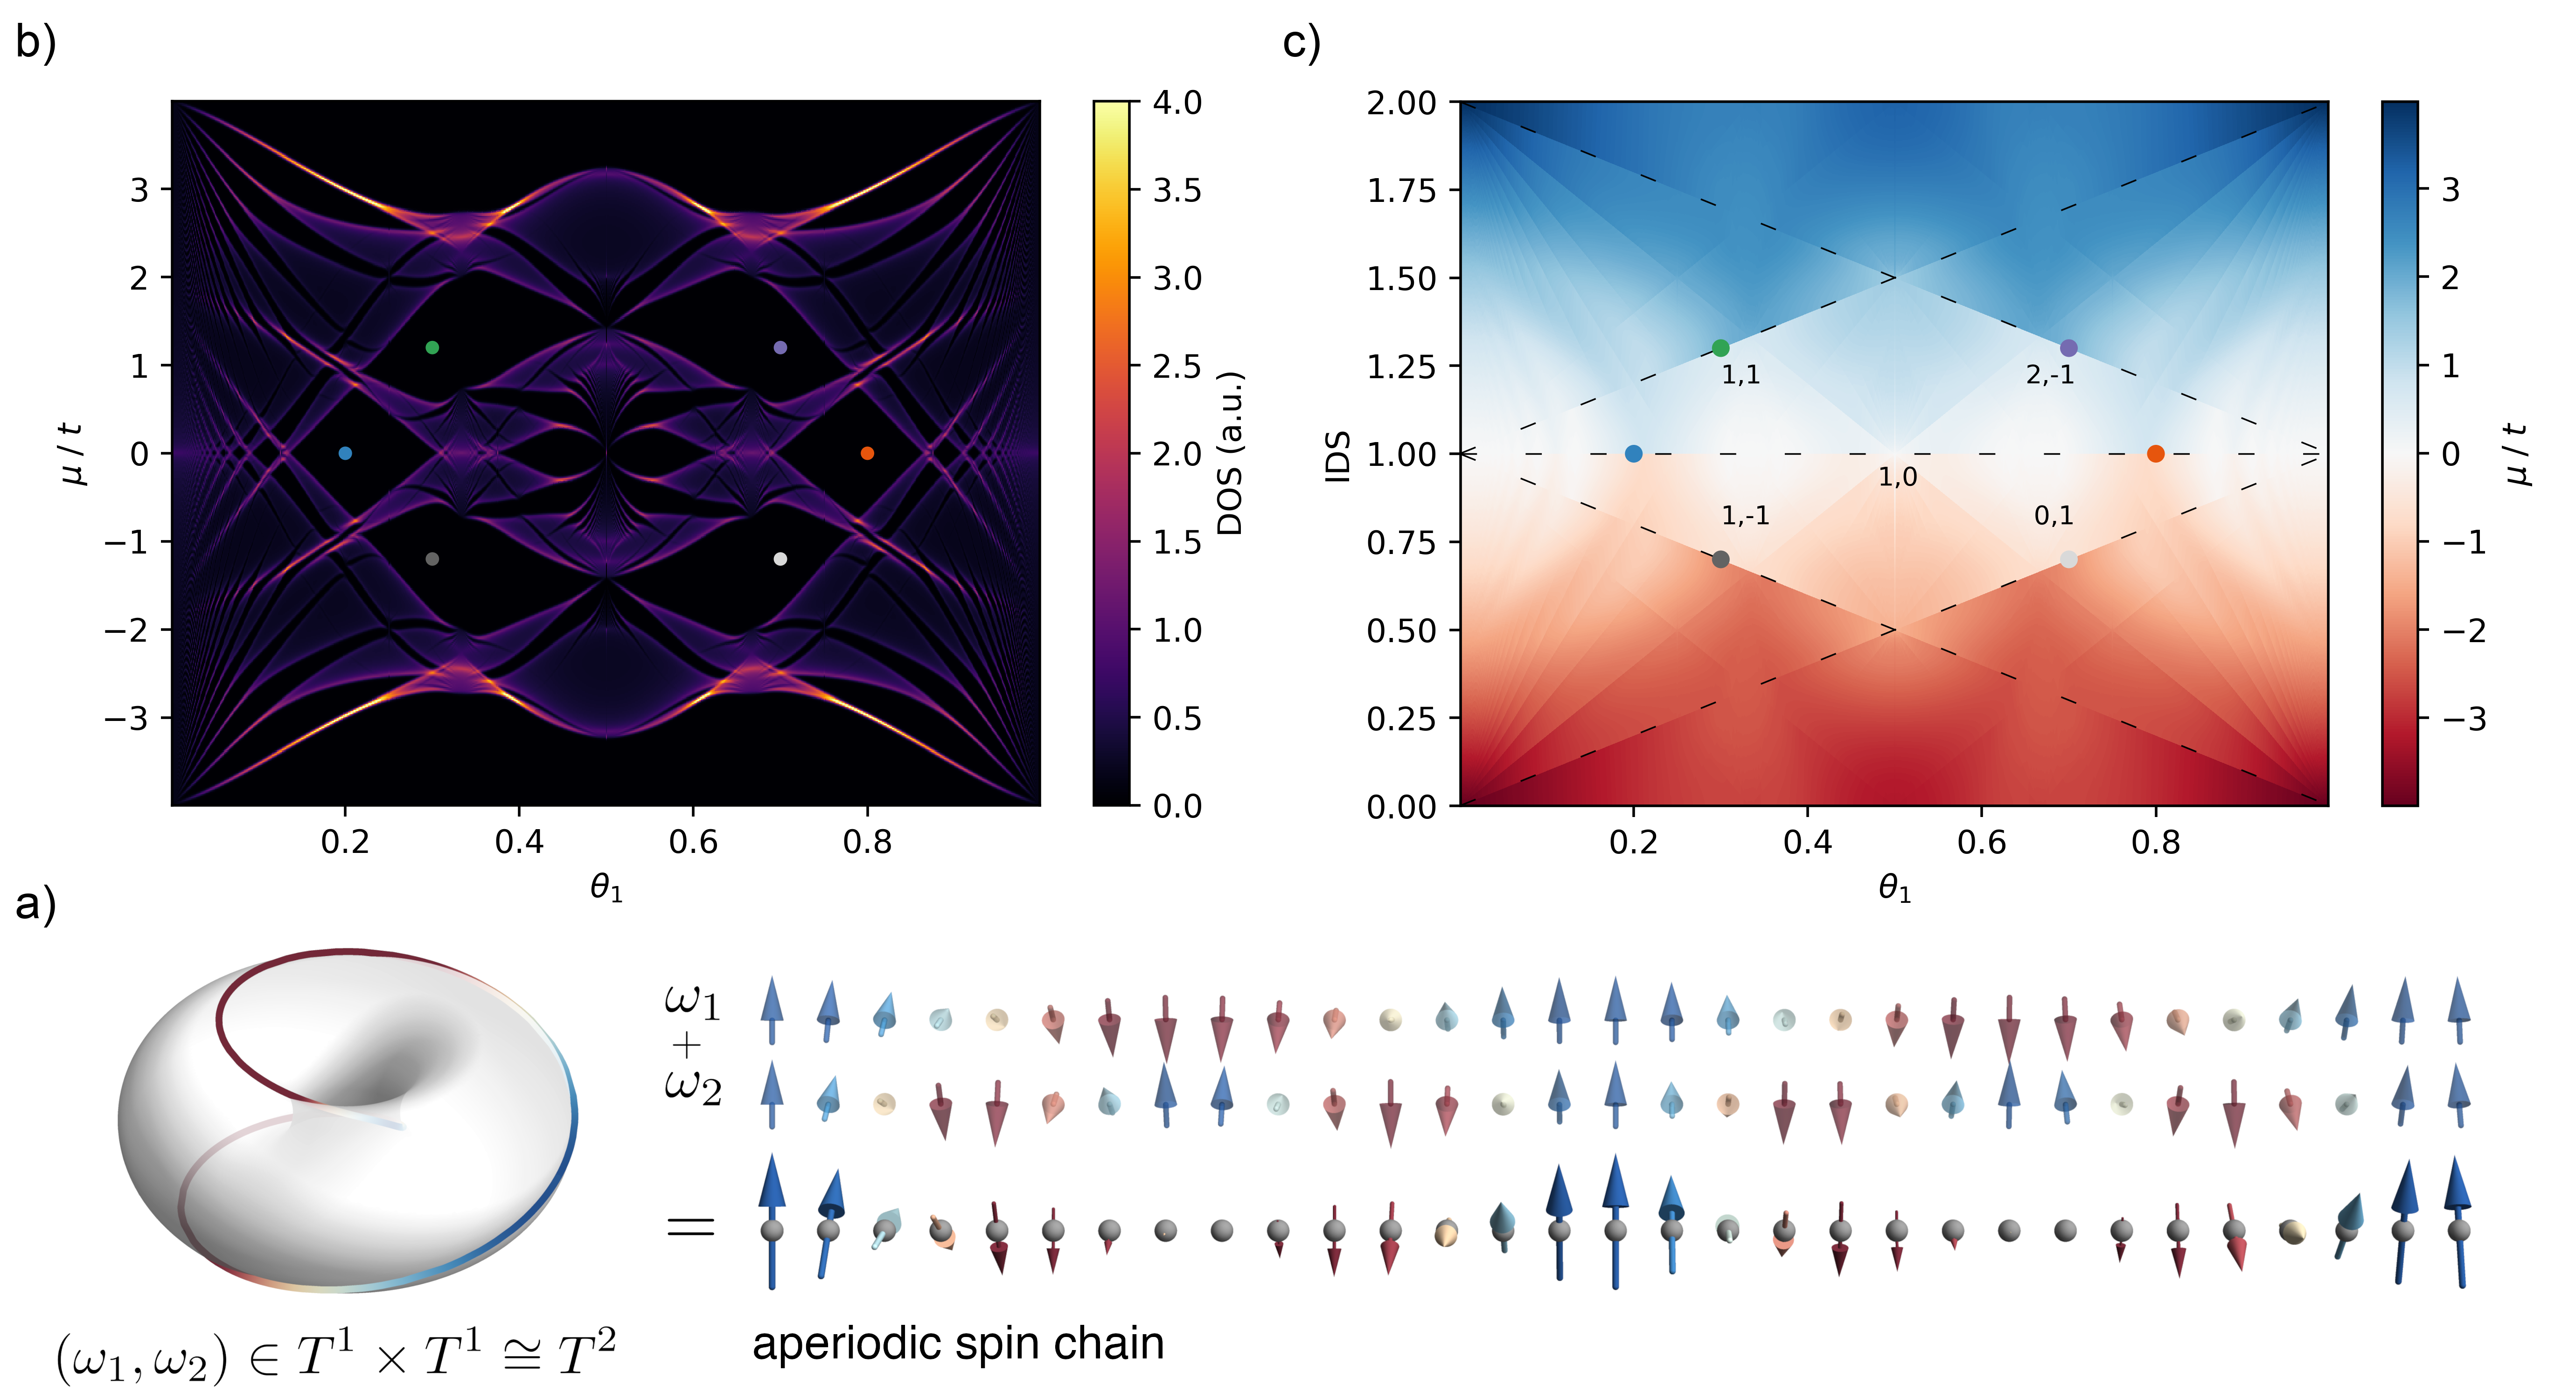
\includegraphics[width=0.8\linewidth]{../gfx/figure_01/figure_01.png}
  \caption{ 
  Fractal spectrum of a spin helix superposition. 
  Fig. a) demonstrates how the superposition of two spin helix states with $\theta_1 = 2\theta_2$.
  Tracing the evolution of individual phase factors $(\omega_1, \omega_2)$ along the lattice generates a path on the 2-torus $T^2$: the hull of the magnetic pattern.
  It is characterized by a nontrivial winding, looping through the hole of the torus.
  We calculate the DOS at $k_\mathrm{B} T = 0.01 t$ and $\xc / t =-1$ for a finite system with $N=1024$ sites and periodic boundary conditions. 
  The values of $\theta_1$ are sampled at rational values $q/N$ with $q\in \mathbb{N}$ and $q \leq N$.
  As the value of $\theta_1$ increases from zero, the spectrum branches into a fractal shape reminiscent of the Hofstadter butterfly.
  Various gaps open in the system, some of them are labeled by the colored bullet points. 
  Each gap can be characterized from the integrated density of states (IDS) in Fig c): the discontinuities in the colormap correspond to gap openings in the spectrum of Fig b). 
  The line features are the characteristic fingerprints of the underlying K-theory description.
  }  
  \label{fig:limacon}
  \end{figure*}

There is however an important subclass of realistic magnetic textures whose spectra are completely characterized by the topological properties of their observable algebras.
Namely, it is not uncommon that such a magnetic texture is described by one or more phase factors through which the real-space dependence will enter the Hamiltonian. 
These are generally known as multi-$\vec{q}$ states and encompass 1D textures such as spin-spirals, but also magnetic skyrmion lattices such as the famous A phase of \ce{MnSi}.
Each multi-$\vec{q}$ texture is characterized by
the presence of $r$ distinct vectors $\vec{q}_i$ with $i=1,\cdots,r$ expressed in terms of the reciprocal lattice as $\vec{q}_i = \sum_{j=1}^d \theta_{ij} \vec{b}_j$.
The dependence on the $\vec{q}$-vectors enters the magnetization texture $\hatn$ via the
phase factors 
$
    \omega_i (\vec{x}_\vec{k}) \equiv  (\vec{x}_\vec{k}  \cdot \vec{q}_i/ (2\pi) + \varphi_i) \mod 1 
$, where $\varphi_i \in \mathbb{R}$ represents a constant phase shift, implying that instead of $\hatn(\vec{x})$  one can write $\hatn( \boldsymbol{\omega} (\vec{x}) )$.
Since $\omega_i \in [0,1) \cong \mathbb{R}/ \mathbb{Z} \cong T^1$, where $T^1$ is the 1D torus, a multi-$\vec{q}$ texture is really a composition of maps: $\mathbb{R}^d \overset{\boldsymbol{\omega}}{\rightarrow} T^r
     \overset{\hatn}{\rightarrow} S^2 $, where $T^r$ is the $r$-dimensional torus.
By inserting the Bravais lattice expansion, one obtains
\begin{equation}
    \omega_i (\vec{x}_\vec{k}) = \left(
      \vec{k} \cdot \boldsymbol{\theta}_i
     + \varphi_i
    \right) \mod 1,
\end{equation}
where $\boldsymbol{\theta}_i$ is the $i$-th row vector of $\theta_{ij}$.
There is also a natural action $\tau$ of the translation group $G=\mathbb{Z}^d$ on these phase factors, given by
$
    \tau_{\vec{m}}\omega_i (\vec{x}_\vec{k}) =\omega_i (\vec{x}_\vec{k} ) - ( \vec{m} \cdot \boldsymbol{\theta}_i \mod 1) ,
$
with $\vec{m}\in \mathbb{Z}^d$ and where the result is to be understood w.r.t. $\mod 1$.
This means that the pattern of phase factors is completely specified by defining the phases  $\boldsymbol{\phi} \equiv \boldsymbol{\omega}(\vec{x}_0) \in T^r$  at one arbitrary, but fixed reference point $\vec{x}_0 \in \mathbb{R}^d$.
The collection of all phase factors which are realized in the system defines {\it the hull} of the magnetic pattern~\cite{Bellissard2000}:
$
    \Omega = G\boldsymbol{\phi}= \lbrace \tau_{\vec{m}}\boldsymbol{\phi} ~|~ \vec{m} \in \mathbb{Z}^d \rbrace  \subset T^r 
$.
If at least one $\theta_{ij}$ is irrational, $\Omega$ forms a dense subset of $T^r$.

%-- observable algebra ----------------------------

Taking this into account, the Hamiltonian $H$ from Eq.~(\ref{eq:hamiltonian}) can now be rewritten in a way, which makes the observable algebra apparent.
The basic idea is to distill the generators of the algebra by formulating $H$ in terms of these.
This can be achieved by casting $H$ into the form~\footnote{For details, we refer to the Supplemental Material}:
\begin{equation}
    H =  \sum_{\vec{i} \in \mathbb{Z}^d} \hat{T}_\vec{i}  \sum_{\vec{j} \in \mathbb{Z}^d} h_\vec{i}( \boldsymbol{\phi} + \theta \vec{j} ) \ket{ \vec{j}} \bra{ \vec{j}} ,
    \label{eq:covariant_hamiltonian}
\end{equation}
where $h\colon T^r \to \mathrm{Mat}_{2\times2} (\mathbb{C}^2)$,
%Intuitively, 
the sum over $\vec{j}$ visits all lattice sites, and the sum over $\vec{i}$ all neighbors.
\revise{
A similar reformulation of the Hamiltonian is also known from the Hofstadter model $H_\mathrm{HF} = t \sum_{\braket{\vec{i},\vec{j}} \in \mathbb{Z}^{2} \times \mathbb{Z}^2}e^{i a_{\vec{i} \vec{j}}} c_\vec{k}^\dagger c_\vec{l} $ describing electrons in a uniform magnetic field in two dimensions~\cite{Hofstadter1976}, where $a_{\vec{k} \vec{l}}$ is the integral of the magnetic vector potential from site $\vec{x}_\vec{l}$ to site $\vec{x}_k$.
This Hamiltonian can be written as $H_\mathrm{HF} = \hat{S}_1 +  \hat{S}_2 + \mathrm{h.c.} $ in terms of the magnetic translation operators $\hat{S}_i = e^{i a_{i+1,i}} \hat{T}_i$~\cite{Zak1964}, where $\hat{T}_i$ to represents a unit lattice translation in direction $i$.
These operators obey the commutation relation $\hat{S}_1 \hat{S}_2 = e^{2\pi i n_\Phi} \hat{S}_2 \hat{S}_1$, where $n_\Phi$ is the number of magnetic flux quanta per unit cell.
The knowledge of this algebraic structure completely characterizes the topological properties of the associated Hofstadter spectrum~\cite{Hofstadter1976, Bellissard1994, Prodan2016}.
}

Eq.~(\ref{eq:covariant_hamiltonian}) now demonstrates, that the observable algebra of the aperiodic spin system is completely determined \revise{(or generated)} by the lattice translation operators and the space of continuous, matrix-valued functions on the torus.
\revise{In other words, any observable can be written in the same generic form as Eq.~(\ref{eq:covariant_hamiltonian}).
We can narrow down on the minimal set of generators: 
by Fourier decomposition, scalar complex functions on the torus $T^r$ are generated by the complex phase factors $u_k = e^{ 2 \pi i \phi_k}$, where $\boldsymbol{\phi} \in T^r $.
Consider now $\tau_i$ to be a unit lattice translation in direction $i$. 
Following the previous definition of the translation operator, we have $ \tau_l \phi_k = \phi_k - \theta_{kl}$  and find}
the commutation relations $ [\tau_i, \tau_j] = 0 $, $ [u_i, u_j]  = 0$ and $\tau_l u_k = e^{-2 \pi i \theta_{kl}} u_k  \tau_l$~\SupplementalMaterial.
By defining $\boldsymbol{\alpha}=(\tau_1, \ldots, \tau_d, u_1,\ldots u_r )$, these relations can be summarized to $\alpha_l \alpha_k = e^{2 \pi i \Theta_{lk}} \alpha_k  \alpha_l$, where
\begin{equation}
    \Theta = \begin{pmatrix}
    0 & -\theta^T \\
    \theta & 0
    \end{pmatrix} .
\end{equation}
The observables of the system can therefore be characterized by the universal $C^\ast$-algebra given by the presentation~\footnote{\revise{The equation uses a common shorthand notation whereby the elements before the $|$-sign are the abstract generators of the algebra and the terms following the $|$-sign are relations these generators have to fulfill.}}
\begin{align}
    \mathcal{A}_\Theta &= \Braket{ \alpha_1, \cdots, \alpha_{r+d}
    |  \alpha_l \alpha_k = e^{ 2 \pi i \Theta_{lk}} \alpha_k  \alpha_l }.
\end{align}
This algebra is known as the \emph{noncommutative torus} in $r+d$ dimensions~\cite{Rieffel1981, Connes1994, Prodan2019}.
\revise{It can be interpreted as a generalization of the algebra describing the Hofstadter model, where $\Theta_{lk}$ now describes generalized magnetic fluxes in the higher-dimensional space with $r$ artificial extra dimensions associated to the $\vec{q}$-vectors~\cite{Kraus2013, Ma2021}}.
%The full observable algebra including spin  is then characterized by the tensor product $\mathcal{A} = \mathcal{A}_\sigma \otimes \mathcal{A}_\theta$, where $\mathcal{A}_\sigma$ is the algebra of hermitian $2\times2$ matrices.

\revise{
Noncommutative K-theory classifies the projection operators which can arise from this observable algebra~\cite{Park2008,Blackadar1998, Connes1994}.
Loosely speaking, two projections operators $P$ and $P'$ belong to the same equivalence class $[P]$ if they are related by a unitary transformation $P' = U P U^\dagger $. 
The set of all $[P]$ defines the so-called $K_0$ group of the algebra $\mathcal{A}_\Theta$.
%Equivalently, one could say that $P$ and $P'$ are equivalent if there exists a continuous path between them.
For the case of $\mathcal{A}_\Theta$, the K-theoretical properties are well-understood~\cite{Prodan2016}.
In particular, one has $K_0( \mathcal{A}_\Theta) = \mathbb{Z}^{2^{r+d-1}}$, which is a compact way of saying that any class of topologically equivalent projection operators $[P]$ can be written as a linear combination of generators $[P] =\sum_J n_J [E_J]$, conveniently labelled by even cardinality subsets $J$ of $\mathcal{I}=\lbrace \tau_1 \cdots, \tau_d, u_1  \cdots, u_r \rbrace$~\SupplementalMaterial.
}

\revise{
For the case when a periodic supercell can be chosen, it is known that the higher-order Chern numbers carry the essential topological information about the physical system~\cite{Qi2008,Kraus2013}.
This concept can be generalized via noncommutative geometry~\cite{Liu2020, Prodan2016}.
If $|J| = 2 m $, ${\rm Ch}_{J} (g) \in \mathbb{N}$ describes a noncommutative $m$-th Chern number, where  ${\rm Ch}_{\emptyset} (g)$ is just the integrated density of states (IDS).
In the lattice periodic case, ${\rm Ch}_{{\tau_1, \tau_2}} (g)$ is nothing but the integral of the momentum space Berry curvature $\Omega_{k_1 k_2}$, while ${\rm Ch}_{{\tau_1, u_1}} (g)$ would translate into an integral over a mixed-space Berry curvature $\Omega_{k_1 \omega_1}$.
Since we have found that the underlying observable algebra $\mathcal{A}_\Theta$ is the noncommutative torus, the Chern numbers have to fulfill~\cite{Prodan2016},
\begin{equation}
   {\rm Ch}_{J'} (g) =  \sum_{J \subseteq \mathcal{I} }^{|J|~\mathrm{even}}  n_J(g) \, {\rm Ch}_{J'}(E_J),
   \label{eq:chern_expansion}
\end{equation}
where ${\rm Ch}_{J'}(E_J)=1$ if $J=J'$,  ${\rm Ch}_{J'}(E_J)=0$ if $J \not\subseteq J'$ and ${\rm Ch}_{J'}(E_J) = \mathrm{Pf}( \Theta_{J\setminus J'})$ otherwise.
This means we can use the IDS to map out some possible Chern numbers which can be realized from the Hamiltonian in Eq.~(\ref{eq:hamiltonian}).
}

% \revise{
% More consequences follow from the fact that $\mathcal{A}_\Theta$ is the noncommutative torus.
% We define the higher-order Chern numbers of the gap $g$ for $J' \subset J$:~\cite{TheNoncommutativeNthChern}
% \begin{equation}
%     {\rm Ch}_{J'}(g) = \frac{(2\pi i)^{|J'|/2}}{( |J'|/2 )!} \sum_{\sigma \in \Ss_{|J'|}} (-1)^\sigma \Tt\Big ( P \prod_{j \in J'} \partial_{\sigma_j}P \Big ),
% \end{equation}
% where $\Tt = \lim_{N\to\infty} N^{-1} \tr~$ is the trace per unit volume and $P$ projects to the occupied subspace of gap $g$.
% Technically, the objects $\partial_{\tau_i}$ and $\partial_{u_j}$ represent derivations on $\mathcal{A}_\theta$ which translate into crystal momentum derivates $\partial_{\tau_i} \to \partial_{k_i}$ and phase derivatives $\partial_{u_j} \to  \partial_{\omega_j}$ when a commensurate supercell can be chosen~\SupplementalMaterial.
% Since we are dealing with $\mathcal{A}_\Theta$, the Chern numbers as defined before have to fulfill~\cite{Prodan2016a},
% \begin{equation}
%    {\rm Ch}_{J'} (g) =  \sum_{J \subseteq \mathcal{I} }^{|J|~\mathrm{even}}  n_J(g) \, {\rm Ch}_{J'}(E_J),
%    \label{eq:chern_expansion}
% \end{equation}
% where ${\rm Ch}_{J'}(E_J)=1$ if $J=J'$,  ${\rm Ch}_{J'}(E_J)=0$ if $J \not\subseteq J'$ and ${\rm Ch}_{J'}(E_J) = \mathrm{Pf}( \Theta_{J\setminus J'})$ otherwise.
% Since ${\rm Ch}_{\emptyset} (g)$ is just the integrated density of states (IDS), we can use it to map out some of the possible Chern numbers which can be realized from the Hamiltonian in Eq.~(\ref{eq:hamiltonian}).
% }
% {\color{blue}
% Noncommutative K-theory classifies the projection operators which can arise from this observable algebra.
% In particular, the $K_0$ group is given by $K_0(\mathcal{A}) = \mathbb{Z}^{2^{r+d-1}}$, which 
% is a compact way of saying that any class of topologically equivalent projection operators $[P]$ can be written as a linear combination of generators $[P] =\sum_J n_J [E_J]$, conveniently labelled by even cardinality subsets $J$ of $\mathcal{I}=\lbrace \tau_1 \cdots, \tau_d, u_1  \cdots, u_r \rbrace$~\SupplementalMaterial.
% The coefficients $n_J$ are necessarily integers, and constitute the full topological characterization of $[P]$~\cite{Prodan2016a}.
% %The coefficients $n_J$ are necessarily integers, which is closely related to the integrality of the Chern numbers \cite{Prodan2016a}
% More familar from the physicists point of view is the notion of the Chern number, here defined as (how to explain this without the notation overhead?)
% \begin{equation}
%     {\rm Ch}_J(P) = \Lambda_J \sum_{\sigma \in \Ss_{|J|}} (-1)^\sigma \Tt\Big ( P \prod_{j \in J} \partial_{\sigma_j}P \Big ),
% \end{equation}
% where $\Tt = \lim_{N\to\infty} N^{-1} \tr~$ is the trace per unit volume and $\Lambda_J=?$.
% For lattice periodic insulators, ${\rm Ch}_{ \lbrace \tau_1, \tau_2 \rbrace } (P)$ is then nothing but the integrated momentum-space Berry curvature. 
% \begin{equation}
%     {\rm Ch}_{\emptyset} (g) =  \sum_{J \subseteq \mathcal{I} }^{|J|~\mathrm{even}}  n_J(g)~\mathrm{Pf}~\Theta_J,
%     \label{eq:chern_expansion}
%  \end{equation}
% }
 
% \revise{Referees find this paragraph too difficult $\rightarrow$ move technical definitions to appendix, rephrase content in more intuitive language}
% Noncommutative K-theory classifies the projection operators which can arise from this observable algebra.
% In particular, the $K_0$ group is given by $K_0(\mathcal{A}) = \mathbb{Z}^{2^{r+d-1}}$, which means that any class of topologically equivalent projection operators $[P]$ can be written as a linear combination of generators $[P] =\sum_J n_J [E_J]$, conveniently labelled by even cardinality subsets $J$ of $\mathcal{I}=\lbrace \tau_1 \cdots, \tau_d, u_1  \cdots, u_r \rbrace$.
% The coefficients $n_J$ are necessarily integers, and constitute the full topological characterization of $[P]$~\cite{Prodan2016a}.
% For a gap projection $g$ on the noncommutative torus, 
% this characterization can be achieved by a computation of the Chern numbers
% $ {\rm Ch}_{J'}$ labelled by $J' \subseteq \mathcal{I}
% $~\cite{Prodan2016a}, i.e.,
% \begin{equation}
%    {\rm Ch}_{J'} (g) =  \sum_{J \subseteq \mathcal{I} }^{|J|~\mathrm{even}}  n_J(g) \, {\rm Ch}_{J'}(E_J),
%    \label{eq:chern_expansion}
% \end{equation}
% where ${\rm Ch}_{J'}(E_J)=1$ if $J=J'$,  ${\rm Ch}_{J'}(E_J)=0$ if $J \not\subseteq J'$ and ${\rm Ch}_{J'}(E_J) = \mathrm{Pf}( \Theta_{J\setminus J'})$ otherwise.
% The operation $\mathrm{Pf}$ denotes the Pfaffian and $\Theta_{J\setminus J'}$ denotes the representation of $\Theta$ in the reduced index set $J\setminus J'$.
% We focus on the zeroth Chern number $ {\rm Ch}_{\emptyset}$, which is nothing but the integrated density of states (IDS)~\cite{Apigo2018}:
% \begin{equation}
%     {\rm Ch}_{\emptyset}(g) = \mathrm{IDS}(g) = \lim\limits_{N\to\infty}  \frac{1}{N} \tr~P_{E<E_g},
%     \label{eq:ids_sum}
% \end{equation}
% where $N$ is the number of lattice sites, $E_g$ is an energy in the gap $g$ and $P_{E<E_g}$ is the projector onto the states below $E_g$.
% In the following, we use the IDS, to map out the possible Chern numbers which can be realized from the Hamiltonian in Eq.~(\ref{eq:hamiltonian}).
% As suggested by Eq.~(\ref{eq:chern_expansion}), multi-$\vec{q}$ magnetism can generate a finite $\Theta$-matrix, and thereby faciliate the emergence of topologically nontrivial electronic states. 

%The IDS therefore encodes topological properties of the spectrum and Eq.~(\ref{eq:chern_expansion}) demonstrates that multi-$\vec{q}$ magnetism can drive distinct topological features in the spectrum, since it generates a finite $\Theta$ matrix.

\begin{figure*}[t]
 \centering
 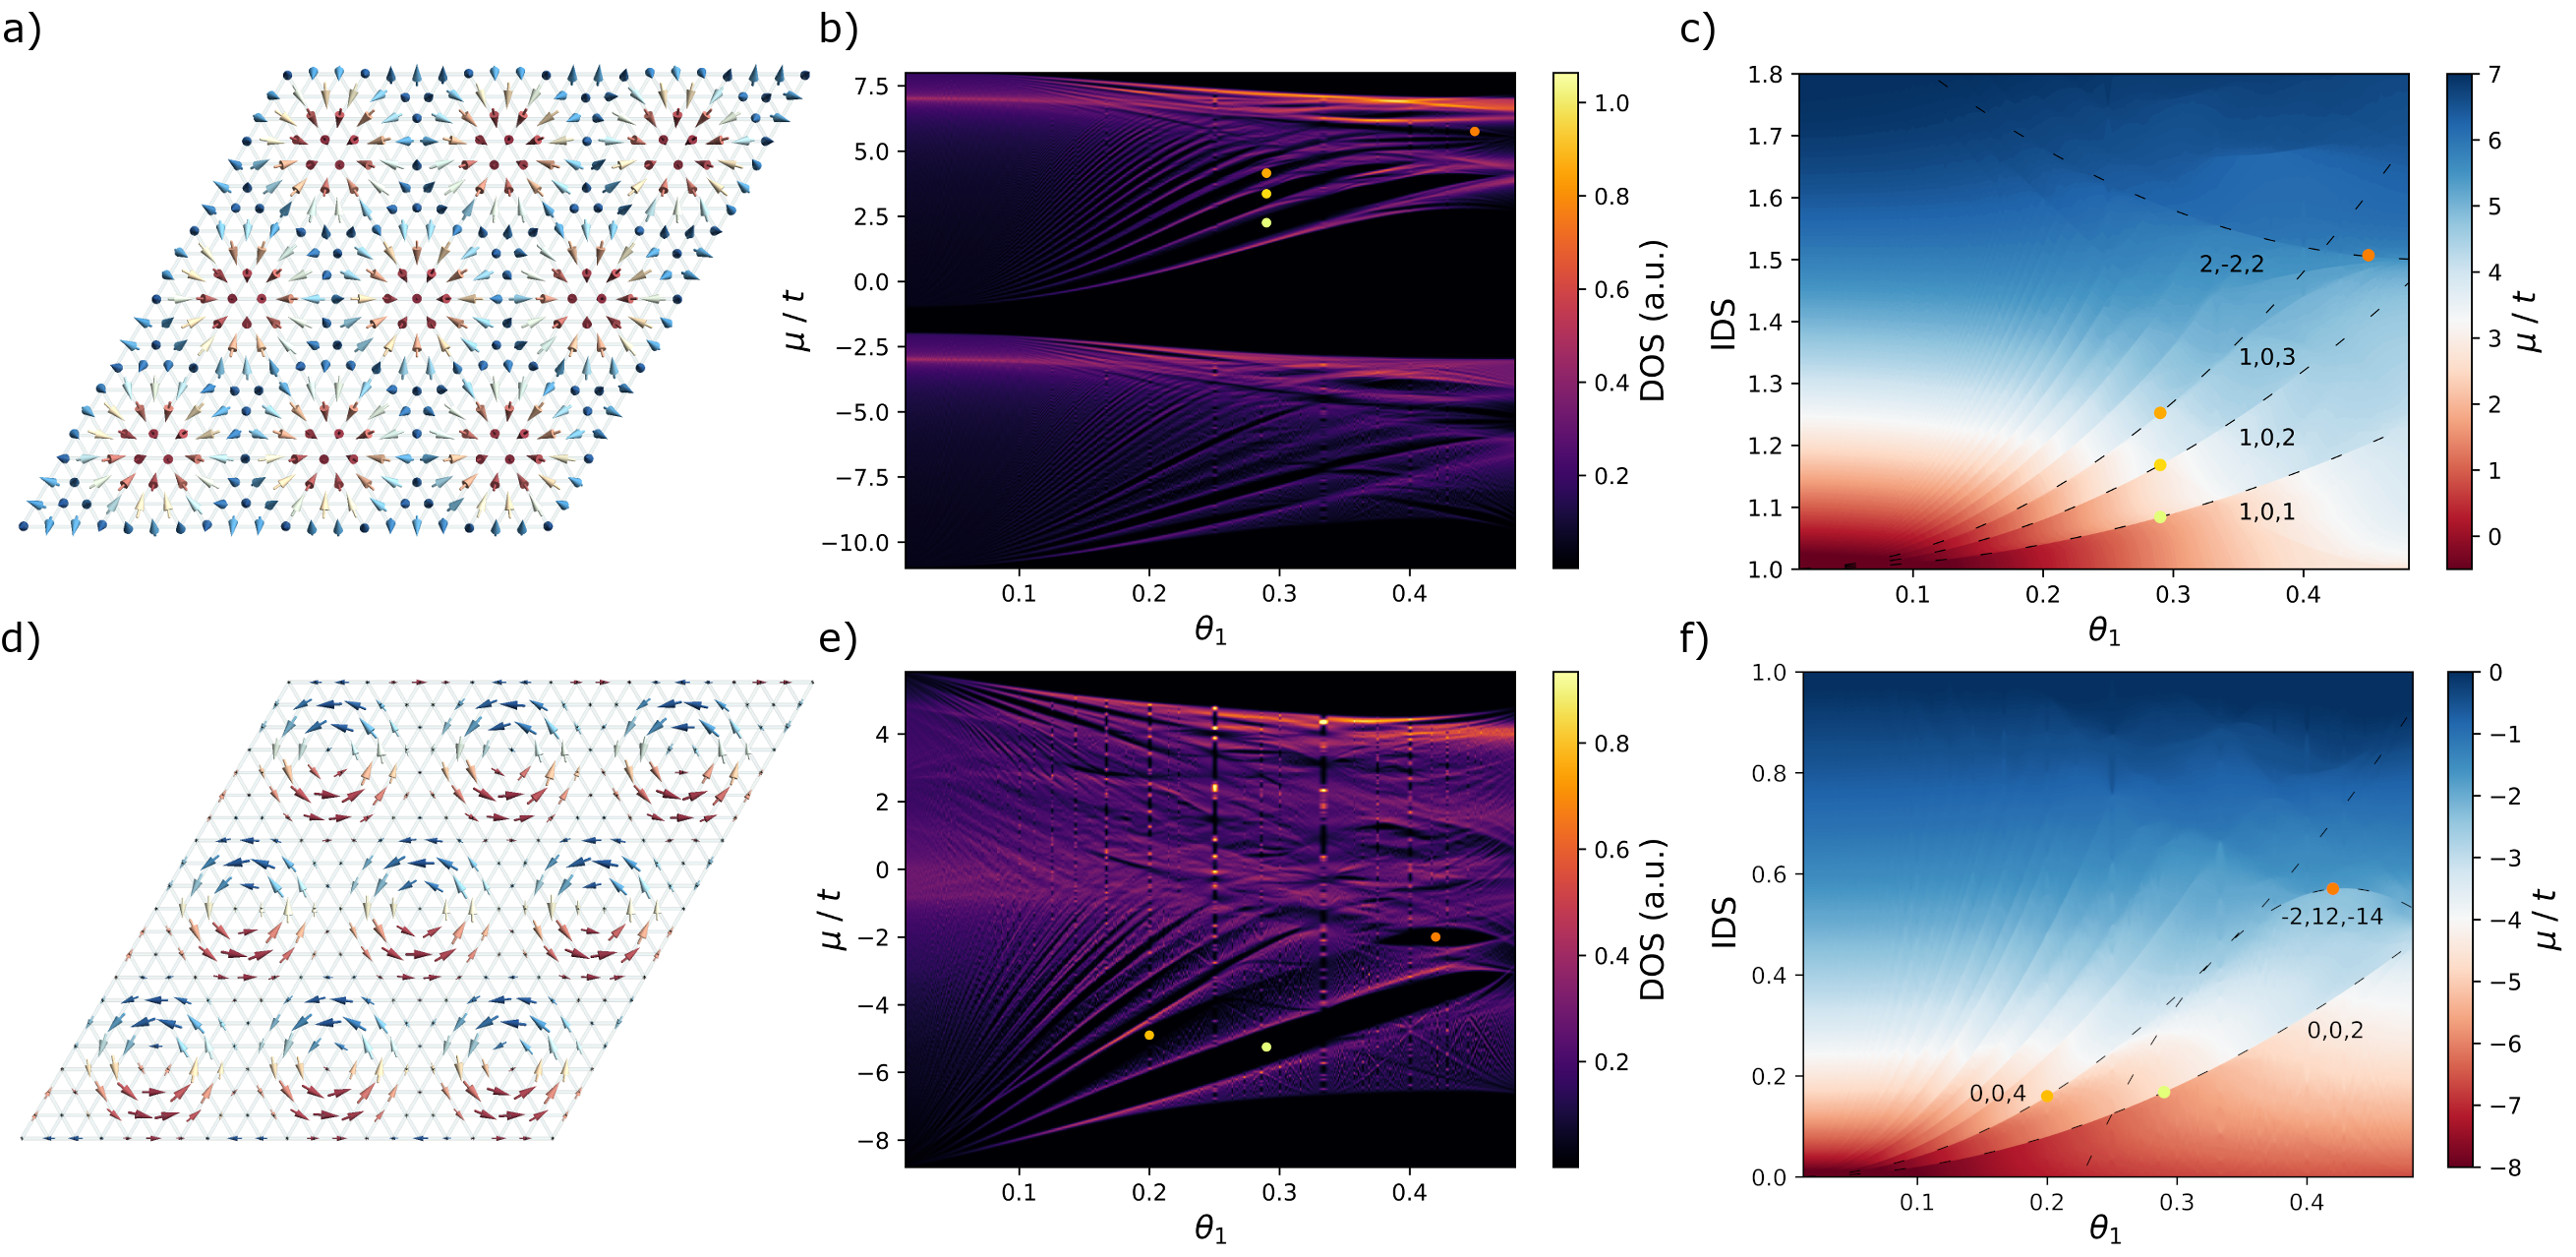
\includegraphics[width=0.85\linewidth]{../gfx/figure_02/figure_02.png}
 \caption{
     Topological spectrum of 3-$\vec{q}$-states.
     Fig a) shows an example for skyrmionic 3-$\vec{q}$-states on the triangular lattice with $N=400$, $\theta_1 = 3/\sqrt{N}$ and periodic boundary conditions.
     The DOS at $k_\mathrm{B}T = 0.01t$, $\xc / t=-5$ is calculated by combining all system sizes $\sqrt{N} \in [19,79]\cap \mathbb{N}$ with  $\sqrt{N}\theta_1 \in \mathbb{Z}$.
     A series of gaps opens in the spectrum (some of them labelled with bullet points) whose topological character is revealed in the IDS plot of Fig c).
     This procedure is repeated for the 3-$\vec{q}$ spin vortex crystal in Fig d).
    Again, the DOS in e) reveals gaps of topological character, as confirmed in f).
    The visible vertical features in e) are due to a reduced sampling density in $\theta_1$ at those points. 
 }  
 \label{fig:three_q_states}
\end{figure*}



%-- limacons --------------------------------------

To illustrate this point, we start with investigating the following superposition of two helicoidal spin spirals ($r=2$):
$\hatn( \boldsymbol{\omega}(x_k ) )
=\sum_{i=1}^{2}( \cos ( 2 \pi \omega_i(x_k) )\vec{e}_y
+\sin ( 2 \pi \omega_i(x_k) )\vec{e}_z)
$,
defined on a 1D lattice ($d=1$) implying $\omega_i(x_k) = k \theta_i + \varphi_i$. 
This system could be realized physically via the proximity coupling of a 1D electronic system to two independent atomic spin spirals, each stabilizing a spin helix \footnote{Another way to think about is as a noncollinear spin density wave.}.
We consider the special case of $\theta_2 = 2 \theta_1$, i.e., $\theta_1$ and $\theta_2$ are rationally dependent \footnote{Other relations between $\theta_1$ and $\theta_2$ could be considered, but will not change the qualitative results, except for $\theta_1=\theta_2$, where the spectrum is trivial.}.
For this situation, the orbit of the lattice translation group generates a dense, 1D subspace on the 2-torus:  $\Omega \cong T^1 \subset T^2$ which is the hull (see Fig. \ref{fig:limacon}).
For the numerical analysis, we consider a finite system of $N=1024$ atoms with periodic boundary conditions. 
The spectrum $\lbrace \epsilon_n \rbrace$ is then calculated by exact diagonalization for different values of $\theta_1$, sampled at rational values $q/N$ with $q\in \mathbb{N}$ and $q \leq N$.
In a first step, we consider the density of states at the chemical potential $\mu$, given by
$\mathrm{DOS}(\mu) = \sum_{n=1}^{2N} \partial_\mu f( \epsilon_n - \mu)$, where $f(\epsilon) = 1/ ( \exp\lbrace \epsilon / (k_B T) \rbrace + 1 ) $ is the Fermi-Dirac distribution.
The result is shown in Fig. \ref{fig:limacon} for different values of $\mu$, and reveals a characteristic Hofstadter butterfly.
As the value of $\theta_1$ is varied, multiple gaps open and close in the spectrum, some of which we label by the colored bullet points.
The topological nature of these gaps can now be investigated by the means of K-theory.
Since the $\theta$-matrix is simply given by $\theta = (\theta_1, 2\theta_1)^T$, the evaluation of the Pfaffian leads to the prediction
\begin{equation}
    \mathrm{IDS}(g) = n_\emptyset(g) + n_{\tau u}(g)~\theta_1 ,
    \label{eq:k_prediction}
\end{equation}
with $n_{\tau u}(g) =  n_{ \lbrace \tau_1, u_1 \rbrace}(g) + 2 n_{ \lbrace \tau_1, u_2 \rbrace}(g) $, where the coefficients can be identified with the first Chern numbers 
$ \mathrm{Ch}_{ \lbrace \tau_i, u_i \rbrace} = n_{ \lbrace \tau_i, u_i \rbrace}$. 
This result can be readily verified by plotting the IDS versus $\theta_1$, color-coded by $\mu$ in Fig.~1.
Since the IDS is constant within a gap, the color exhibits discontinuous jumps which makes it possible to track the evolution of IDS for a specific gap as a function of $\theta_1$.
The result is in perfect agreement with Eq.~(\ref{eq:k_prediction}), and makes it possible to assign a unique label $(n_\emptyset, n_{\tau u})$ to each gap $g$.
Since the gaps with $n_{\tau u} \neq 0$ are characterized by a nontrivial first Chern number, the superposition of spin helices leads to a topologically nontrivial spectrum.


%-- skyrmions and vortices ---------------------------------

One way to interpret the $\Theta$ matrix of $\mathcal{A}_\Theta$ is to think of it as a generalized magnetic flux.
This is similar to the emergent field of smooth magnetic skyrmions~\cite{Bliokh2005, Schulz2012}, but is a more far-reaching generalization of this concept, which also makes sense for discrete systems.
To investigate the transition into the conventional emergent field picture, we consider a triangular lattice with $\vec{a}_1 = a (1,0)^T$, $\vec{a}_2 = a (1/2,\sqrt{3}/2 )^T$ and reciprocal lattice vectors
$\vec{b}_1 = 2 \pi (1, -1/\sqrt{3})^T / a$, $	\vec{b}_2 = 2 \pi (0, 2 / \sqrt{3})^T / a$.
With respect to this lattice, we devise a $\theta$-matrix
$ \theta = \theta_1 (( 
	0, 1),
	(  1,0 ),
	( -1,-1 )) $,
which corresponds to the coherent superposition of three spin spirals~\SupplementalMaterial. 
This gives rise to a 3-$\vec{q}$ skyrmion lattice shown in Fig. \ref{fig:three_q_states}a) with the K-theory prediction
\begin{equation}
     \mathrm{IDS}(g) = n_\emptyset(g) + n_{\tau u}(g)~\theta_1 + n_{\tau^2u^2}(g)~\theta_1^2,
    \label{eq:k_prediction_skx}
\end{equation}
where $n_{\tau u} = n_{ \lbrace \tau_1 , u_2\rbrace} + n_{\lbrace\tau_1 , u_3\rbrace}+n_{\lbrace\tau_2 , u_1\rbrace}+n_{\lbrace\tau_2 , u_3\rbrace}$ and $n_{\tau^2u^2} = n_{\lbrace\tau_1, \tau_2 , u_1 , u_2\rbrace} +  n_{\lbrace\tau_1 , \tau_2 ,  u_1 ,  u_3\rbrace} + n_{\lbrace\tau_1 , \tau_2 ,  u_2  , u_3 \rbrace}$.
We proceed similarly as for the spin helices and calculate $\mathrm{DOS}(\theta_1)$ and $\mathrm{IDS}(\theta_1)$ for different system sizes~\SupplementalMaterial.
A series of topological gaps appear in Fig.~\ref{fig:three_q_states}b) as $\theta_1$ is increased away from $0$, which can be classified by the label $(n_\emptyset, n_{\tau u}, n_{\tau^2u^2})$.
The $\theta_1^2$ dependence of the gap sizes  has been theoretically observed for the skyrmion lattice~\cite{Hamamoto2015} and now finds its explanation as a fingerprint of the underlying K-theory.
According to the classification of Fig.~\ref{fig:three_q_states}c), 
these gaps correspond to a quantization of $n_{\tau^2u^2}$ with $n_{\tau u}=0$.
Naively, this seems to indicate that the first Chern numbers are zero which would be in contradiction to the known quantized topological Hall effect in this system.
However, the anomalous Hall effect picks up the different Chern number $\mathrm{Ch}_{ \lbrace \tau_1 \tau_2 \rbrace } = n_{ \lbrace \tau_1 \tau_2 \rbrace }$ \cite{Prodan2017} which is not visible in the IDS.
In the adiabatic limit $m/t \to \infty$ and $\theta_1 \to 0$, it can be shown that $\mathrm{Ch}_{ \lbrace \tau_1 \tau_2 \rbrace } = n_{\tau^2u^2}$~\SupplementalMaterial, and the apparent contradiction is resolved.
Noteworthy, these results persist as $\theta_1$ approaches the scale of the underlying lattice, since the respective gaps can be continuously connected to the limit of $\theta_1 \to 0$.
Here (and in particular for gaps which are not connected to the adiabatic limit), any arguments based on the smoothness of the texture fail, while the K-theory description can still be upheld.

To further underline this point, we perform the same calculation after replacing the superposition of spin spirals by a superposition of spin density waves which gives rise to the spin texture in Fig.~\ref{fig:three_q_states}d)~\SupplementalMaterial. 
In this case, it is not obvious what the emergent field language would predict, and  
in fact, the emergent magnetic field in the continuous limit  $B_\mathrm{em} = \hatn \cdot(\partial_x \hatn \times \partial_y \hatn)$ is vanishing for this texture.
Manifestly, with the K-theory description, no such conceptual problems arise.
The $\theta$-matrix is not changed as compared to the previous case and the prediction for the IDS as the marker of topologically nontrivial electronic states in this system is valid. 
It is thus of no surprise that topological gaps are visible in the DOS in Fig.\ref{fig:three_q_states}d), while the associated IDS in Fig.~\ref{fig:three_q_states}e) is again in perfect agreement with the K-theory of multi-$\vec{q}$ order.
This serves to show that the generalized fluxes $\Theta$ can provide a connecting theme which extends to more exotic magnetic phases such as vortex crystals in frustrated magnets~\cite{Wang2015}.

%-- Conclusion ------------------------------

To summarize, in this work we put forward a new method to characterize electronic topological states emerging in real-space spin textures which is based on the K-theory of $C^\ast$-algebras.
In contrast to conventional methods of topological characterization based on smooth Berry phase properties such as the emergent field of skyrmions or Berry curvature of Bloch states $-$ whose meaning is lost in aperiodic, disordered or non-smooth textures $-$ the K-theory analysis can be used to predict and understand the appearance of nontrivial gaps in generic spin systems even of the latter kind. 
As such, the K-theory categorization bears great promise for unraveling and shaping the hybrid topological properties of electronic states in complex spin textures which can be realized in realistic samples. 
Particular exciting aspects to address in the future are the topology of three-dimensional textures which have the potential to harvest six-dimensional physics (nontrivial third Chern numbers are a theoretical possibility for the 3$\vec{q}$ cubic hedgehog lattice~\SupplementalMaterial), as well as the K-theory topological interpretation of spin fluctuations, dynamical excitations of real-space spin systems and the associated edge state physics.

\vfill \newpage

%-- acknowledgements ------------------------------

We  acknowledge  funding  under SPP 2137 ``Skyrmionics'' (project  MO  1731/7-1)  of  Deutsche  Forschungsgemeinschaft (DFG) and also gratefully thank the J\"ulich Supercomputing Center and RWTH Aachen University for providing computational resources under project jiff40. 
This work was further supported by the Max Planck Graduate Center with the Johannes Gutenberg-Universit\"at Mainz (MPGC).
Emil Prodan acknowledges financial support from the W.M. Keck Foundation and USA National Science Foundation through grant  DMR-1823800.


%-- literature ------------------------------------

\hbadness=99999 
\bibliographystyle{apsrev4-2}
\bibliography{literature}

\end{document}

